\lesson{13}{09/04/2020} Now we would like to know the frequency at which we have to re-balance our portfolio in order to follow the fluctuations of the underlying. This is given by the Greek $\Gamma$.

\subsection{Gamma} % riascolta se hai tempo
The gamma ($\Gamma$) of a portfolio of options on an underlying asset is the rate of change of the portfolio's delta with respect to the price of the underlying asset. It is the second partial derivative of the portfolio with respect to asset price:
\begin{equation}
    \Gamma = \pdv[2]{price}{S} = \pdv{\Delta}{S} = \dfrac{1}{S\sigma\sqrt{T-t}}\dfrac{e^{-\frac{d_1}{2}}}{\sqrt{2\pi}}.
\end{equation}
If gamma is small, the delta changes slowly and adjustments to keep a portfolio delta-neutral need to be made only relatively infrequently. If gamma is highly negative or highly positive, the delta is very sensitive to the price of the underlying asset and it is quite risky to leave a delta-neutral portfolio unchanged for any length of time.
\begin{figure}[htp]
    \centering
    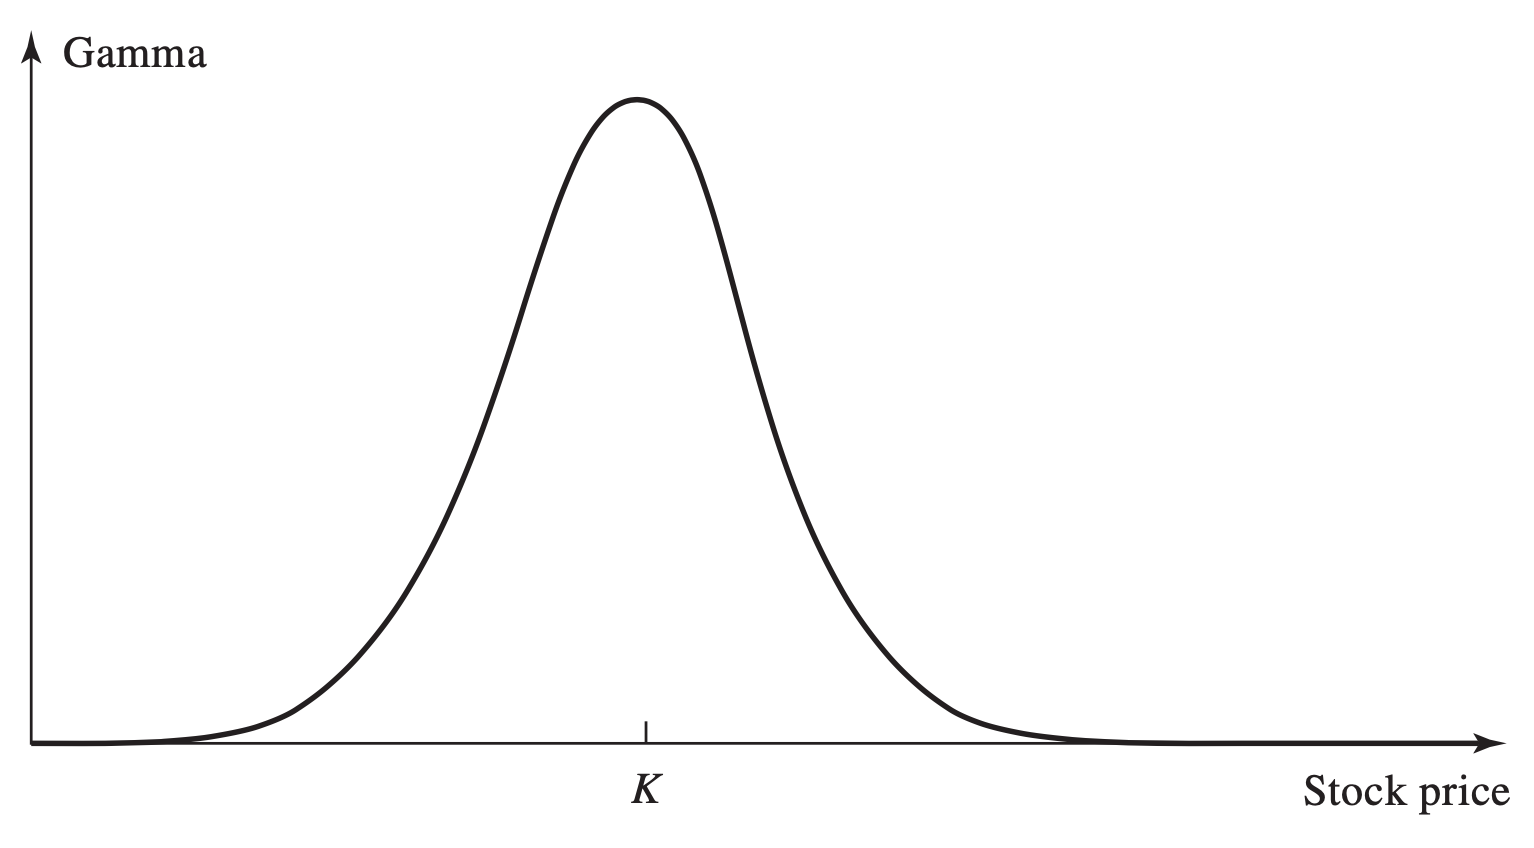
\includegraphics[scale=0.2]{fig/tmp/fig14.png}
    \caption{Variation of gamma with stock price for an option.}
    \label{fig:gamma}
\end{figure}

\subsection{Rho}
The rho of a portfolio of options is the rate of change of the value of the portfolio with respect to the interest rate:
\begin{equation}
    \rho = \pdv{price}{r} = K(T-t)e^{-r(T-t)}\Phi(d_2).
\end{equation}
It measures the sensitivity of the value of a portfolio to a change in the interest rate when all else remains the same. Notice that it is not normalized as the delta.
\begin{figure}[htp]
    \centering
    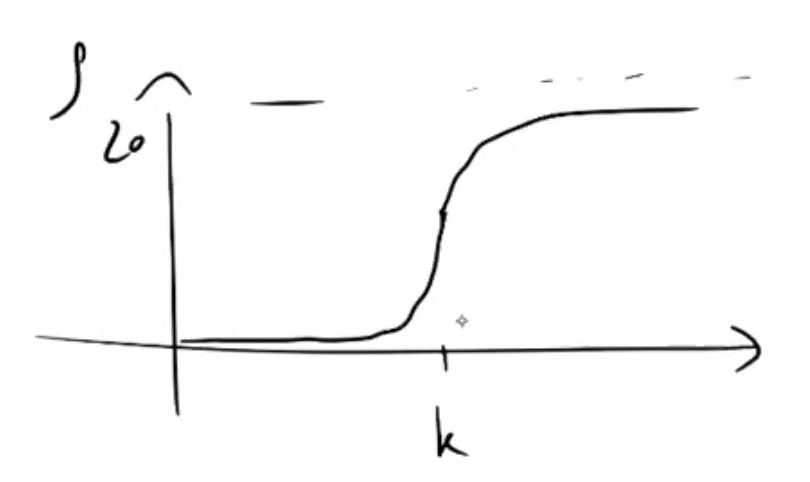
\includegraphics[scale=0.3]{fig/tmp/fig15.png}
    \caption{Variation of rho with stock price for an option.}
    \label{fig:rho}
\end{figure}
\newline Its interpretation is that if we are far from the strike, a bias in the estimation of the interest rate is not a problem. Conversely, if we are around the strike a small bias in the estimation of the interest rate results in a huge change in the price.

\subsection{Theta}
The theta ($\Theta$) of a portfolio of options is the rate of change of the value of the portfolio with respect to the passage of time with all else remaining the same. Theta is sometimes referred to as the \emph{time decay} of the portfolio.
\begin{equation}
    \Theta = \pdv{price}{t} = \dfrac{-S\sigma e^{-\frac{d_1^2}{2}}}{4\sqrt{2\pi(T-t)}}-rKe^{-r(T-t)}\Phi(d_2).
\end{equation}
Theta is usually negative for an option. This is because, as time passes with all else remaining the same, the option tends to become less valuable (we loose the opportunity to get a greater payoff). The variation of $\Theta$ with stock price for a call option is shown in Figure \ref{fig:theta}.
\begin{figure}[htp]
    \centering
    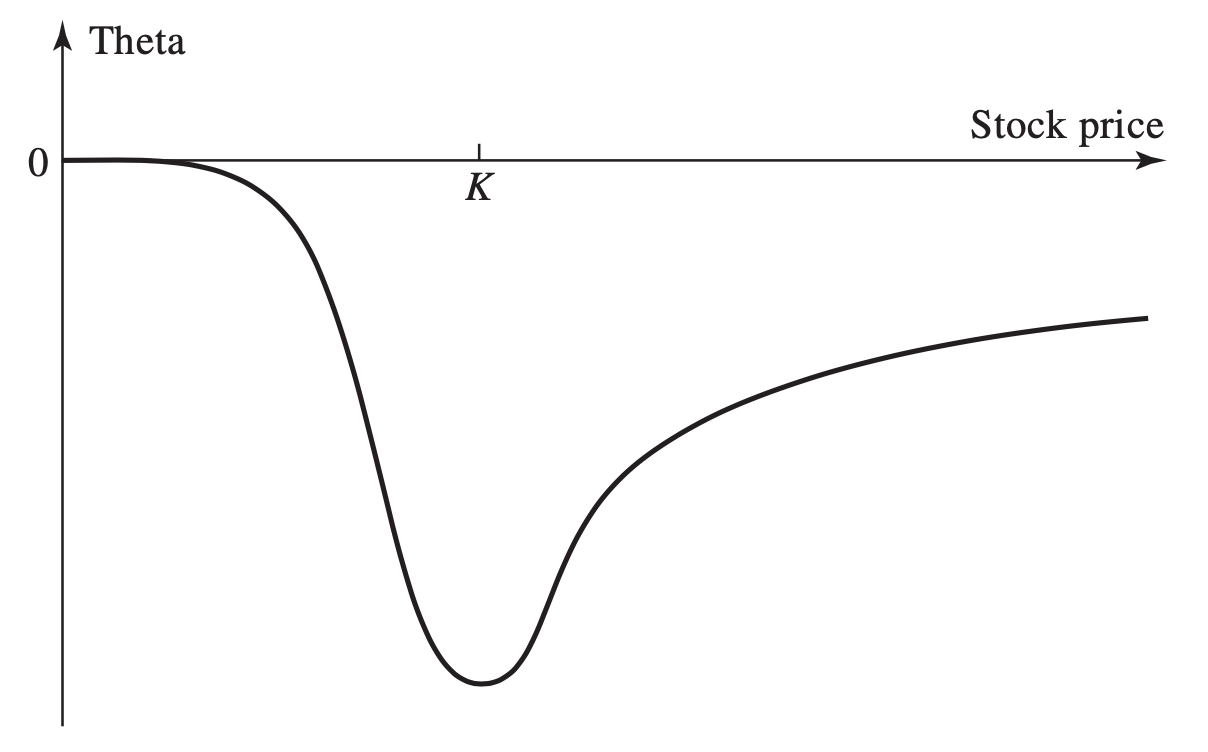
\includegraphics[scale=0.2]{fig/tmp/fig16.png}
    \caption{Variation of theta of a European call option with stock price.}
    \label{fig:theta}
\end{figure}
\newline When the stock price is very low, theta is close to zero. For an at-the-money call option, theta is large and negative. As the stock price becomes larger, theta tends to $-rKe^{-rT}$.

\subsection{Vega}
Up to now we have implicitly assumed that the volatility of the asset underlying a derivative is constant. In practice, volatilities change over time. This means that the value of a derivative is liable to change because of movements in volatility as well as because of changes in the asset price and the passage of time.\\
The vega of a portfolio of derivatives, $\mathcal{V}$, is the rate of change of the value of the portfolio with respect to the volatility of the underlying asset:
\begin{equation}
    \mathcal{V} = \pdv{price}{\sigma}.
\end{equation}
If vega is highly positive or highly negative, the portfolio’s value is very sensitive to small changes in volatility. If it is close to zero, volatility changes have relatively little impact on the value of the portfolio.
\begin{figure}[htp]
    \centering
    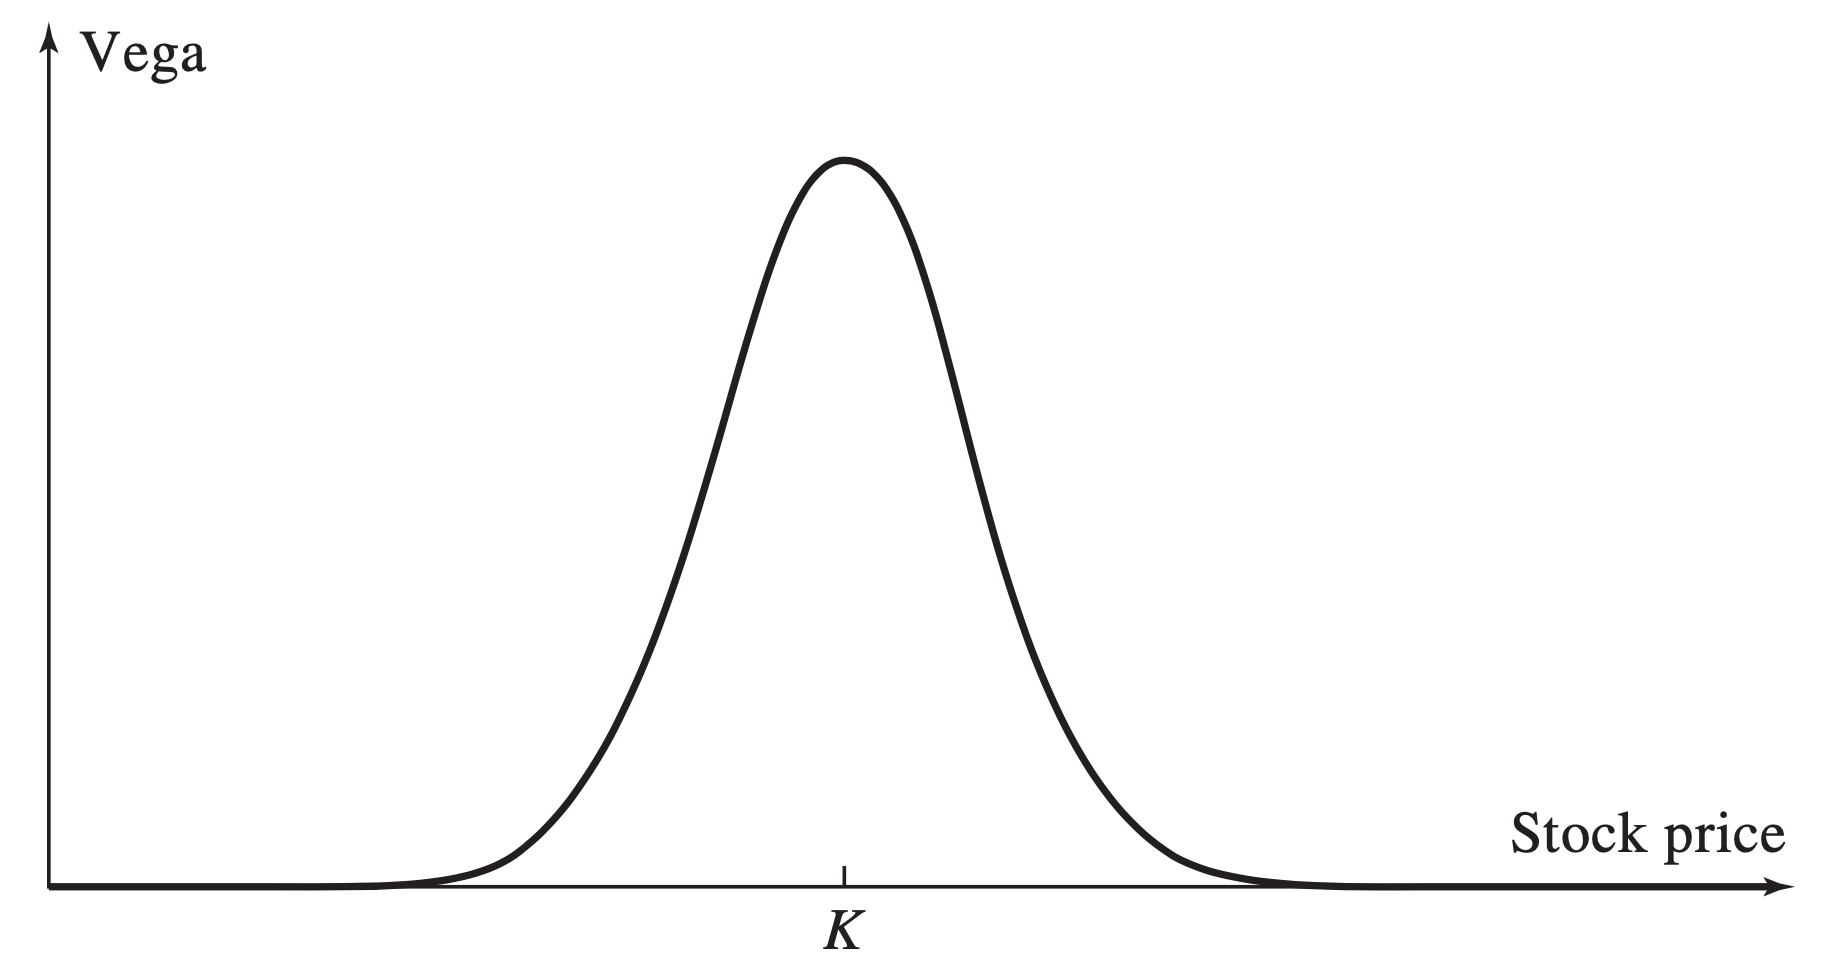
\includegraphics[scale=0.2]{fig/tmp/fig17.png}
    \caption{Variation of vega with stock price for an option.}
    \label{fig:vega}
\end{figure}
\newline The fact that $\mathcal{V}>0$ means that there is a monotone increasing relationship between price and volatility. In other words, the higher the volatility of the option, the higher the price of the option. We can exploit this relationship to invert the B\&S formula and find the volatility in terms of the price. Let us fix the maturity $T$ and suppose that we want to price a set of options indexed by different strikes $K_1,\dots,K_n$: $$B\&S(S,T-t,r,K_1,\sigma),\dots,B\&S(S,T-t,r,K_n,\sigma).$$
Now, if we consider the quoted prices
$$mkt(S,T-t,K_1),\dots,mkt(S,T-t,K_n)$$
we can look for the value of the volatility -- called \emph{implied volatility} -- to plug in the B\&S formula in order to obtain this prices. If the B\&S model is correct we should get always the same value of $\sigma_{imp}$, but indeed in practice we find non-constant values. This distortion is known as \emph{smile effect} and it is the proof that the B\&S model is not 100\% correct.
\begin{figure}[htp]
    \centering
    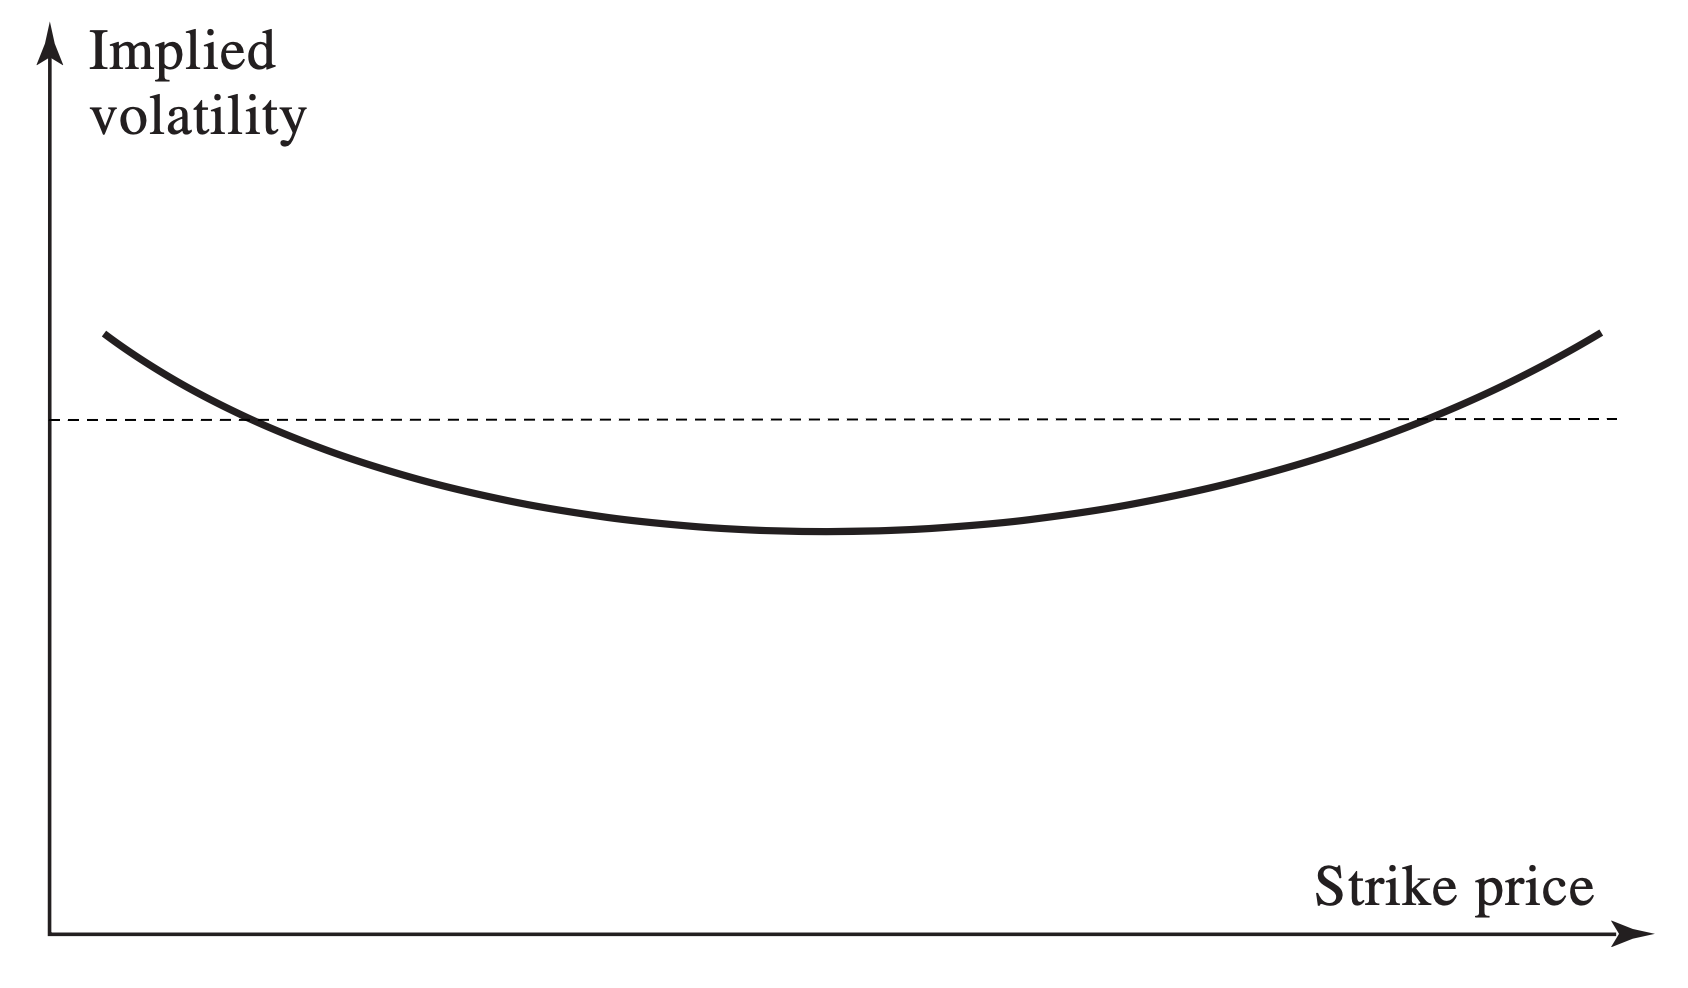
\includegraphics[scale=0.2]{fig/tmp/fig18.png}
    \caption{Smile effect.}
    \label{fig:smile}
\end{figure}
\newline However, the B\&S is very useful because it allows to quote the options not in dollars but in terms of the implied volatility.\\
The form of the smile is very important because it tells us how much the B\&S model is wrong. If the smile is flat it means that the B\&S model is not so wrong, while if it is more pronounced it means that it is dangerous to approximate prices using it.\\
The B\&S model is important also because in some contract there is not a quoted price, so it must be deduced.\\
If we consider different values of the maturity $T$ and we introduce the time to maturity as an additional dimension, we can find the so called \emph{implied volatility surface}. Typically, for short times to maturity the smile is very pronounced (the violation of the B\&S model is stronger) and for longer times to maturity the smile flattens (because of the central limit theorem).
\begin{figure}[htp]
    \centering
    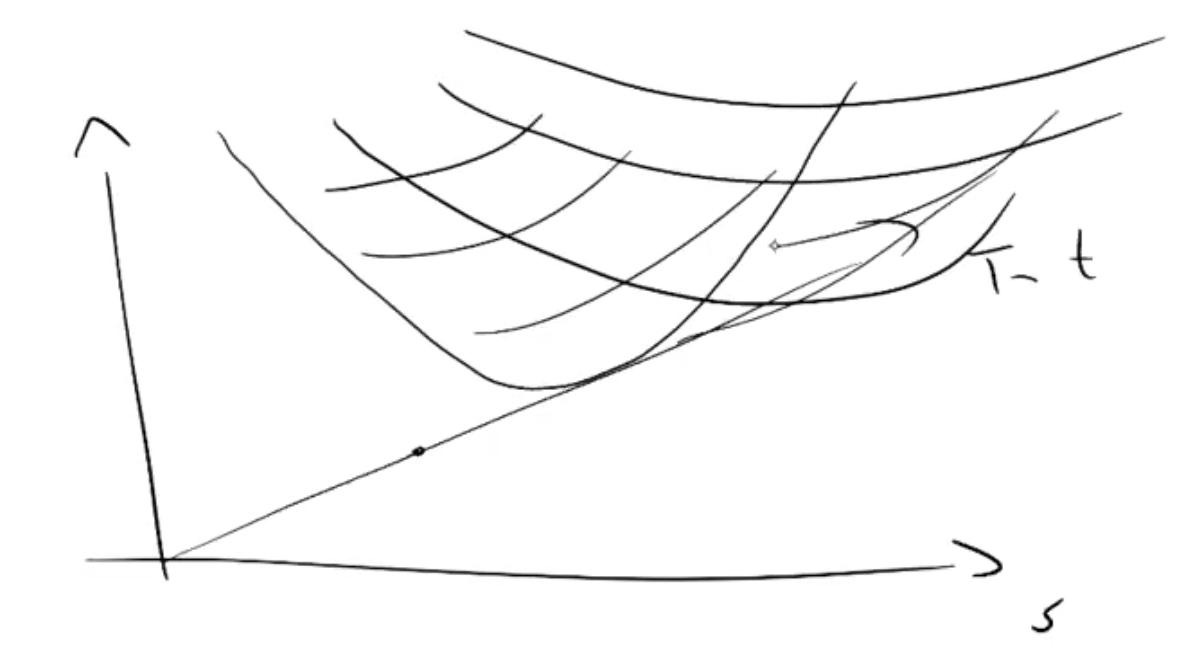
\includegraphics[scale=0.3]{fig/tmp/fig19.png}
    \caption{Implied volatility surface.}
    \label{fig:implvolsurf}
\end{figure}

\subsection{Put option pricing in the Black \& Scholes model}
From the put-call parity we have that:
\begin{align}
    \notag \text{Put}_t &= \call_t + Ke^{-r(T-t)} - S_t \\
    &=
    \notag S_t\Phi(d_1) - Ke^{-r(T-t)}\Phi(d_2) + Ke^{-r(T-t)} - S_t \\
    &=
    Ke^{-r(T-t)}\underbrace{(1-\Phi(d_2))}_{>0} - S_t\underbrace{(1-\Phi(d_1))}_{>0}.
\end{align}
Now we want to understand how to hedge a put option, in particular to find the Greeks. We have:
\begin{equation}
    \Delta^{\text{Put}} = \pdv{\text{Put}_t}{S} = \Phi(d_1)-1.
\end{equation}
In this case the delta of the put is always negative, as we can see in Figure \ref{fig:delta} (b). We also have
\begin{equation}
    \Gamma^{\text{Put}} = \Gamma^{\call},
\end{equation}
\begin{equation}\label{vegaput}
    \mathcal{V}^{\text{Put}} = \mathcal{V}^{\call}.
\end{equation}
Eq. \eqref{vegaput} is very important because it says that the price of the put is an increasing function of the corresponding volatility. This means that we can repeat the procedure of inverting the formula of the price of the put in terms of the volatility in order to get the quoted market price. Even in this case we will have the smile effect.\\
\textbf{What happens to the Greeks and to the price if there is an upward shift in the volatility?} Consider a call option. In any case there are the constraints to start from zero and to converge to the straight line $(S_t-K)^+$. Then we know that for higher volatility we will have higher prices. So, for $\sigma_2>\sigma_1$ the curve will stay above the original price.
The delta will change such that it will be convenient to buy the underlying earlier and to sell it immediately after the strike.
\begin{figure}[htp]
    \centering
    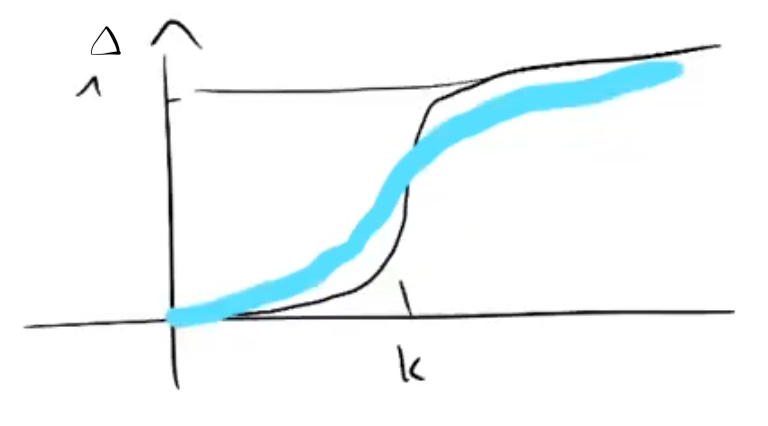
\includegraphics[scale=0.3]{fig/tmp/fig21.png}
    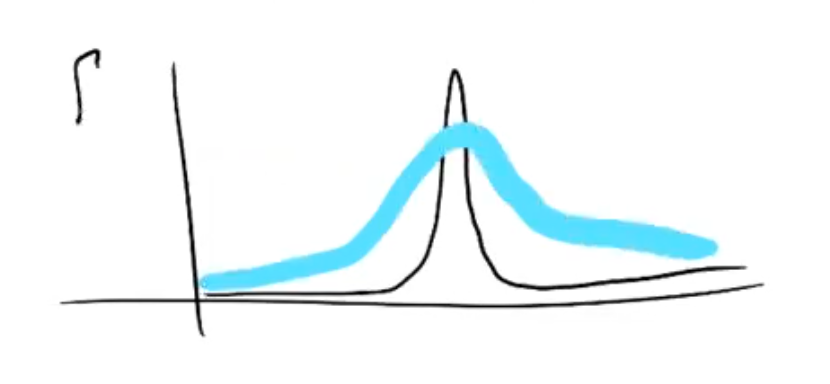
\includegraphics[scale=0.3]{fig/tmp/fig22.png}
    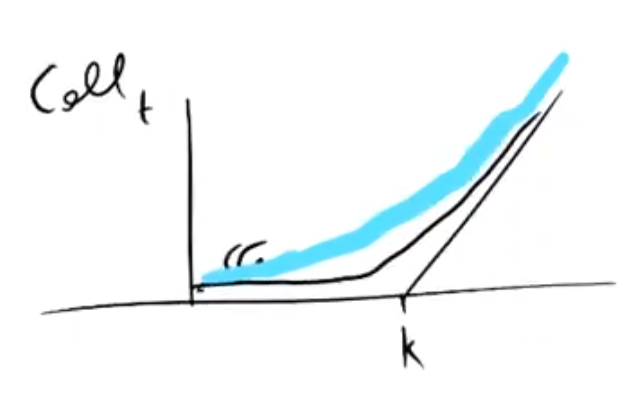
\includegraphics[scale=0.3]{fig/tmp/fig20.png}
    \caption{Delta, gamma and price of a call option for $\sigma_1$ (in black) and $\sigma_2>\sigma_1$ (in blue).}
    \label{fig:call2}
\end{figure}
If the gamma corresponding to $\sigma_1$ was like a Dirac delta, the one for $\sigma_2$ will be more spread out.\\
In other words, there is a smoothing effect both on the price and on the Greeks.

\section{Portfolio immunization}
We would like our portflio to be $\Delta$-neutral, i.e. we would like the global delta of our hedging strategy to match exactly the global delta of the corresponding portfolio derivatives. However, immediately after we balanced the portfolio, there can be a shock in the market. In other words, there is no guarantee for us to stay with the same hedging portfolio for too long. In order to stay safe for a while we need our portfolio to be $\Gamma$-neutral, so that the re-balance frequency is low. Moreover, since the volatility is a crucial ingredient we would like our portfolio to be also $\mathcal{V}$-neutral.\\
For example, from the B\&S PDE
\begin{equation}
    \pdv{F}{t} + rS\pdv{F}{S} + \frac{1}{2}\sigma^2S^2\pdv[2]{F}{S} = rF
\end{equation}
we can replace the derivatives with the corresponding Greeks:
\begin{equation}
    \Theta + rS\Delta + \frac{1}{2}\sigma^2S^2 \Gamma = r\, price.
\end{equation}
For a $\Delta$-neutral portfolio ($\Delta = 0$) we have
\begin{equation}
    \Theta + \frac{1}{2}\sigma^2S^2 \Gamma = r\, price.
\end{equation}
From this equality we immediately understand that if $\Theta<0$ then $\Gamma>0$, which is true for \emph{vanilla options} (call/put). Conversely, if $\Gamma<0$ then $\Theta>0$, which typically happens to \emph{exotic options}. In order to understand what does it mean to have a $\Gamma<0$, let's start from the dynamics of the hedging portfolio:
\begin{equation}
    \dd price_t = \Theta\,\dd t + S\Delta\,\dd S + \frac{1}{2}\sigma^2\Gamma\,\dd S^2.
\end{equation}
Notice that this is a quadratic function of $\dd S$. If $\Gamma$ is positive it means that for large variations of the underlying -- i.e. shocks in the market -- there is no risk (the hedging portfolio leads to a positive P\&L\footnote{The \emph{profit and loss} (P\&L) statement is a financial statement that summarizes the revenues, costs, and expenses incurred during a specified period, usually a fiscal quarter or year. The P\&L statement is synonymous with the income statement. These records provide information about a company's ability or inability to generate profit by increasing revenue, reducing costs, or both.}), whereas for small variations we can incur in some potential risk (negative P\&L). If $\Gamma<0$ we have the converse: for small variations of the underlying there is no risk (positive P\&L) whereas for large variations we can incur in some risk (negative P\&L).
\begin{figure}[htp]
    \centering
    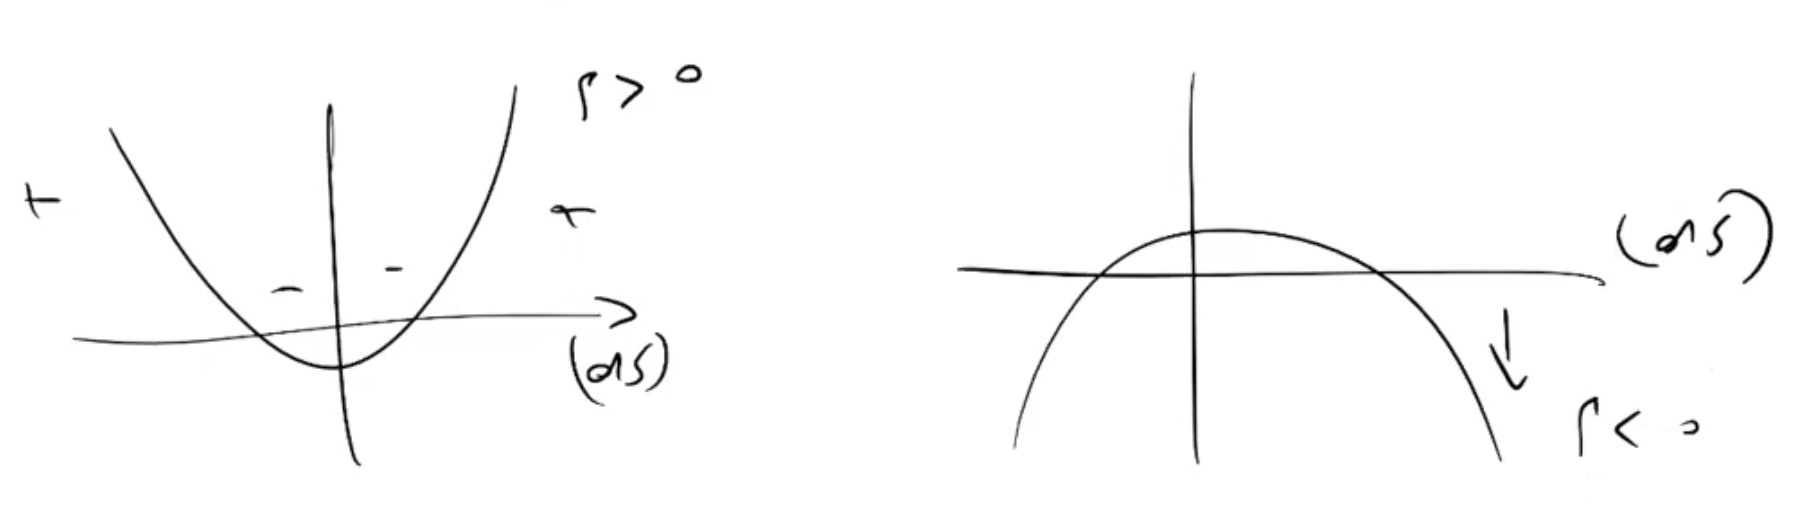
\includegraphics[scale=0.3]{fig/tmp/fig23.png}
    \caption{Hedging portfolio price for (a) $\Gamma>0$ and (b) $\Gamma<0$.}
    \label{fig:pnl}
\end{figure}
\newline Now let's construct an immune portfolio. At the end of the trading day the value of our portfolio is $V_t$ and the corresponding delta is $\Delta^V_t$. If $\Delta^V_t\gg0$ or $\Delta^V_t\ll0$ there is a mismatch between the behavior of what we are trying to hedge and our corresponding hedging strategy, known as \emph{delta risk}. We have to look for an instrument in the market that allows us to neutralize the global delta. There are two possibilities:
\begin{itemize}
    \item Buy/sell options (put, call, \dots). In the immunization we have to take into account their prices;
    \item Consider linear contracts (forward contract, futures, \dots). Since we do not have to pay in order to enter these contracts, these are cheaper strategies. These are delta-1 products, i.e. their delta is 1. In fact, if we consider as an example a long position in a forward contract, we have that the payoff is $S_T-K$ and according to the risk neutral methodology its price is
    \begin{align*}
        price_t^{\fwd} &= e^{r(T-t)}\mathbb{E}^\Qmeas[S_T-K]\\
        &=
        e^{rt}\mathbb{E}^\Qmeas[e^{-rT}S_T] - Ke^{r(T-t)} \\
        &=
        e^{rt}e^{-rt}S_t - Ke^{-r(T-t)} \\
        &=
        S_t - Ke^{-r(T-t)},
    \end{align*}
    so the delta is $\Delta^{\fwd}_t=1$.
\end{itemize}
Let's consider the situation in which $\Delta^V_t\ne0$ and we take a position in the forward market entering a contract with maturity $T$ and strike $K$, so that
\begin{equation}
    V^{tot}_t = V_t + \alpha\fwd(T,K),
\end{equation}
\begin{equation}
    \Delta_t^{tot} = \Delta_t^V + \alpha\Delta^{\fwd} = \Delta_t^V + \alpha\cdot 1.
\end{equation}
If we impose $\Delta_t^{tot}=0$ in the last equation we have that the number of forward contracts we have to include in our portfolio is
\begin{equation}
    \alpha = -\Delta^V_t.
\end{equation}
Furthermore, if we want also to neutralize the portfolio with respect to the \emph{gamma risk} (related to the frequency of re-balancing) then linear contracts are useless, because their second derivative with respect to $S$ is zero and so $\Gamma=0$. The idea is to take a position in the options market. The portfolio will be
\begin{equation}
    V^{tot}_t = V_t + \alpha\fwd_t + \beta \call(T,K)
\end{equation}
and we have to jointly impose the delta and gamma neutrality. In fact, if we take the previous $\Delta$-neutral portfolio and we impose the $\Gamma$-neutrality, the involved call option will have $\Delta^{\call}\ne0$ so the neutrality is destabilized. In other words, we have to solve
\begin{equation}
    \begin{cases}
    0 = \Delta^{tot}_t = \Delta_t^V + \alpha + \beta\Delta^{\call}_t \\
    0 = \Gamma^{tot}_t = \Gamma^V_t + 0 + \beta \Gamma^{\call}_t.
    \end{cases}
\end{equation}
If we want also vega-neutrality we have to consider a second option, different from the first (for example with different strike).
